\chapter{Methodology} \label{ch:Methodology}
The core of this research is the development of a modeling framework designed to determine optimal allocation strategies for Battery Energy Storage Systems (BESS). Unlike conventional cost-minimization models that assume a central planner, this work adopts a game-theoretic perspective to capture the strategic interactions between competing private entities. Within this framework, four strategic investors compete across a five-node network for market share and limited grid connection capacity. The optimization is conducted over a representative day with an hourly resolution, accurately internalizing long-term capital expenditures by scaling them to daily costs.

This chapter outlines the core methodology of the thesis, presenting the Equilibrium Problem with Equilibrium Constraints used to model strategic BESS allocation. It sequentially details the underlying Mathematical Programs with Equilibrium Constraints, the integration of technical and economic model expansions, the chosen algorithmic solution strategy, and finally the empirical parameters configuring the test system.

\section{Equilibrium Problem with Equilibrium Constraints}

\begin{figure}
    \centering
    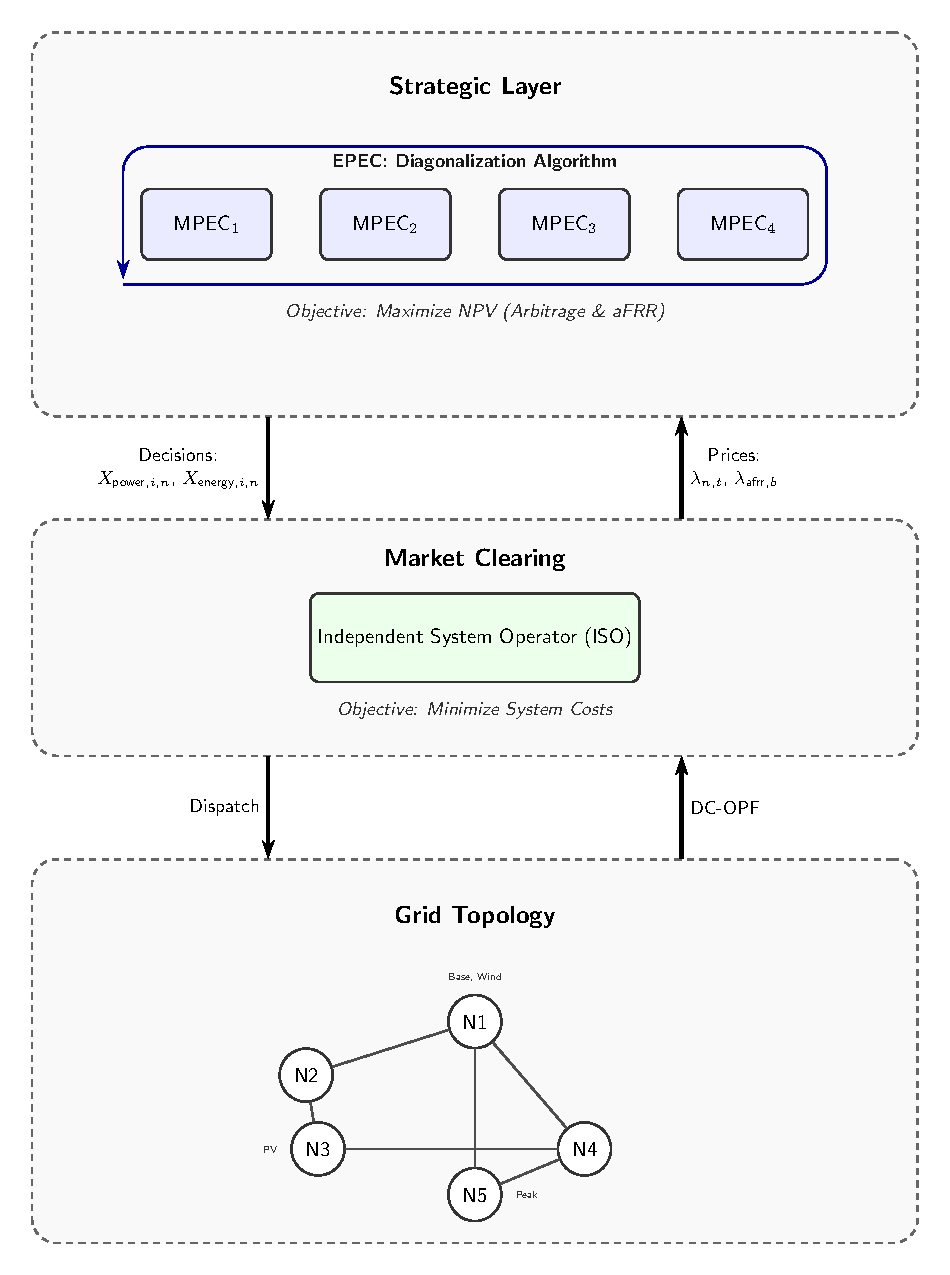
\includegraphics[width=0.75\linewidth]{figures/Lead_Figure.pdf}
    \caption{Modeling approach of BESS investors as strategic agents (MPEC) coupled in their equilibria (EPEC).}
    \label{fig:mpec_epec}
\end{figure}

The mathematical structure employed is an \textbf{Equilibrium Problem with Equilibrium Constraints (EPEC)}. An EPEC is fundamentally a "game" played between multiple strategic leaders who all face a common follower \cite{conejo_complementarity_2020}. In the context of this thesis, the EPEC represents the simultaneous competition of several BESS investors for market share and grid connection capacity.

As shown in Figure \ref{fig:mpec_epec}, the EPEC is composed of several interrelated \textbf{Mathematical Programs with Equilibrium Constraints (MPECs)}, where each MPEC represents the decision-making process of a single strategic investor. Because the objective function of each investor depends not only on their own decisions but also on the investment and operational choices of their rivals, these MPECs are intrinsically coupled \cite{conejo_complementarity_2020}.

Each individual MPEC is structured as a bi-level optimization problem, reflecting a Leader-Follower (Stackelberg) relationship.
\begin{itemize}
    \item \textbf{Upper Level (The Leader)}: This level represents the strategic BESS investors. Their primary goal is to maximize their individual Net Present Value (NPV). The decision variables at this level are the investment choices: the power capacity (\(X_{power}\)) in MW and the energy capacity (\(X_{energy}\)) in MWh to be installed at specific nodes within the grid.
     \item \textbf{Lower Level (The Follower)}: This level represents the Independent System Operator (ISO) or market clearing mechanism. The ISO performs a cost-minimal DC Optimal Power Flow (DC-OPF), ensuring that the system's power balance and technical grid constraints -- such as line limits -- are respected while meeting demand.
\end{itemize}

The levels are coupled through the Locational Marginal Prices (LMPs): the ISO clears the market, and the resulting nodal prices are fed back to the Upper Level, where they determine the revenues and thus the profitability of the investors' BESS assets.

The investors in this model are characterized as strategic agents who act according to the principle of economic rationality. This means each investor assumes that all other market participants (rivals and the ISO) will also act to maximize their own objectives. To ensure this behavior is mathematically captured, the Lower Level market clearing is replaced by its KKT optimality conditions. These conditions are then embedded as constraints within the investors' Upper Level optimization, forcing the strategic actors to internalize the market's response to their investment decisions \cite{conejo_complementarity_2020}.
A defining property of these strategic actors is their heterogeneous risk affinity, which is represented through individual discount rates (\(r_{i}\)). In this framework:
\begin{itemize}
    \item A lower discount rate (e.g., \(r=0.08\)) represents a more "patient" or risk-neutral investor willing to accept longer amortization periods to secure market shares, such as in the capacity-heavy aFRR market.
    \item A higher discount rate (e.g., \(r=0.15\) or \(0.20\)) represents a more risk-averse investor who demands faster returns on investment, typically focusing on high-spread arbitrage opportunities in the spot market.
\end{itemize}

Finding a solution to an EPEC involves identifying a Nash Equilibrium, a state where no single investor can increase their profit by unilaterally changing their investment strategy. Given the non-linear and non-convex nature of coupled KKT conditions, the model is solved via an iterative diagonalization algorithm \cite{conejo_complementarity_2020}.
In this process, the MPEC of one investor is solved while the investment decisions of all other rivals are kept fixed. The algorithm cycles through all investors sequentially (Gauss-Seidel) or in parallel (Gauss-Jacobi) until the changes in investment decisions between iterations fall below a defined tolerance threshold, signifying that a stable equilibrium has been reached.

\section{Upper Level: The Strategic Investor} \label{sect:Upper_Level}
At the Upper Level, each strategic investor \(i\in I\) aims to maximize their individual NPV on a daily operational basis. The primary decision variables are the endogenously determined investment choices for power capacity (\(X_{power,i,n}\)) in MW and energy capacity (\(X_{energy,i,n}\)) in MWh at each node \(n \in N\).
The objective function maximizes the discounted profit from spot market arbitrage trading minus the specific per-day annualized capital expenditures (CAPEX) for power and energy capacity:
\begin{equation}
        \max_{X_{power}, X_{energy}} NPV_{i} = \sum_{t, n} \left[ \lambda_{n, t} \cdot (P_{discharge, i, n, t} - P_{charge, i, n, t}) \right] - CAPEX_{daily, i}  
\end{equation}

To correctly internalize the CAPEX into the daily optimization loop, the investment costs are annualized using the Capital Recovery Factor (CRF). The CRF is calculated over the project lifetime (e.g., 15 years) utilizing the investor-specific discount rate ($r_i$):
\begin{equation}
    CRF_{i} = \frac{r_i \cdot (1+r_i)^{Lifetime}}{(1+r_i)^{Lifetime} - 1}
\end{equation}

The total investment cost is multiplied by the CRF and divided by the days of the year (365.25) to yield the exact daily CAPEX constraint:
\begin{equation}
    CAPEX_{daily, i} = \frac{CRF_i}{365.25} \cdot \sum_{n} (C_{power} \cdot X_{power, i, n} + C_{energy} \cdot X_{energy, i, n})
\end{equation}

The investment decision is subject to several constraints:
\begin{enumerate}
    \item \textbf{Shared Resource Constraint}: The total BESS power capacity installed at any given node \(n\) is restricted by a physical connection limit. Each investor must account for the fixed decisions of their rivals (\(X_{power,j,n}^{fixed}\)):
    \begin{equation}
        X_{power, i, n} + \sum_{j \neq i} X_{power, j, n}^{fixed} \le Limit_n
    \end{equation}
    
    \item \textbf{Energy-to-Power Ratio}: To ensure technical feasibility and align with typical battery configurations, a minimum ratio between energy and power capacity is enforced:
    \begin{equation}
             X_{energy, i, n} \ge Ratio_{min} \cdot X_{power, i, n}
    \end{equation} \label{eq:E_P_Ratio}
    
    \item \textbf{Equilibrium Constraints}: The investor's strategy is constrained by the response of the market clearing mechanism. This is mathematically integrated by including the KKT conditions of the Lower Level problem as constraints within the Upper Level.
\end{enumerate}

\section{Lower Level: Market Clearing} \label{sect:Lower_Level}
The Lower Level represents the ISO, who performs a market clearing to minimize the total dispatch costs of the conventional generators \(g\in G\) over the time steps \(t\in T\).

The objective function is defined as:
\begin{equation}
    \min \sum_{t, g} MC_g \cdot P_{gen,g, t}
\end{equation}

The market clearing process is subject to physical grid and technical storage constraints:
\begin{enumerate}
    \item \textbf{Nodal Power Balance}: At each node \(n\) and hour \(t\), the conventional generation, available wind/PV feed-in, and battery discharge must equal the nodal demand, net exports, and battery charge. The dual variable of this constraint represents the Locational Marginal Price (\(\lambda_{n,t}\)):
    \begin{equation}
        \sum_{g \in G_n} P_{gen,g,n,t} + P_{wind/pv,n,t} + \sum_{i} (P_{discharge, n, t} - P_{charge, n, t}) - D_{n, t} - \text{NetExport}_{n, t} = 0
    \end{equation}

    \item \textbf{Transmission Constraints}: To accurately represent physical power flows within the meshed network, the model employs a linearized DC Optimal Power Flow (DC-OPF) formulation. By utilizing a Power Transfer Distribution Factor matrix (\(PTDF_{l,n}\)), the active power flow on each transmission line \(l\) is computed directly from the net power injections at every node \(n\). To ensure grid security, the resulting flow is strictly bounded by the predefined thermal transmission capacity limit (\(Limit_{l}\)):
    \begin{equation}
        \begin{split}
            NetInjection_{n, t} = \sum_{g \in G_n} P_{gen, g, n, t} + P_{wind/pv, n, t} + \sum_{i} (P_{discharge, i, n, t} - P_{charge, i, n, t}) - D_{n, t} \\
            Flow_{l, t} = \sum_{n \in N} PTDF_{l, n} \cdot NetInjection_{n, t} \\
            |Flow_{l, t}| \le Limit_l \\
        \end{split}
    \end{equation}

    \item \textbf{Generator Limits}: Conventional generators are constrained by their maximum physical capacity: 
    \begin{equation}
        0 \le P_{gen, g, t} \le P_{max, g}
    \end{equation}

    \item \textbf{Storage Technical Equations}: The operation of the BESS is restricted by the capacities chosen at the Upper Level (\(X_{power},X_{energy}\)) and governed by the State of Charge (SOC) balance equation, which accounts for the round-trip efficiency (\(\eta\)):
    \begin{equation}
        \begin{split}
            0 \le P_{charge} \le X_{power} \\
            0 \le P_{discharge} \le X_{power} \\
            SOC_{t} = SOC_{t-1} + \eta \cdot P_{charge,t} - \frac{1}{\eta} \cdot P_{discharge,t} \\
            0 \le SOC_{t} \le X_{energy} \\
            SOC_{t=0} = SOC_{t=24}
        \end{split}
    \end{equation}
    
    \end{enumerate}

\section{Model Expansions: Bridging the Research Gap} \label{sect:Model_Expansions}
The systematic taxonomy developed in Section \ref{sec:soa_bess} identified critical gaps in existing BESS allocation models. While most models optimize BESS purely for day-ahead spot market arbitrage, real-world profitability heavily relies on multi-service market participation and is simultaneously constrained by physical asset degradation. To bridge this gap, the base MPEC was expanded to incorporate both battery degradation and the co-optimization of the spot and Automatic Frequency Restoration Reserve (aFRR) markets. To make the market more realistic, economic RES curtailment for negative prices was added.
However, introducing these complex operational realities into a mathematical EPEC requires careful technical compromises to maintain solvability.
\subsection{Battery Degradation}\label{subsect:Battery_Degradation}
Battery life is significantly impacted by charge and discharge cycles. The literature review demonstrated that omitting degradation leads to overestimating the NPV, as intelligent operational strategies that minimize cyclic stress can substantially defer capital expenditure. Therefore, cycling costs must be internalized in the investor's objective function.

To incorporate this, the Upper Level objective function is adapted by subtracting the degradation costs (\(Cost_{degrad}\)) from the investor's operational revenues. Degradation is modeled as a linear marginal cost applied to the energy throughput. The specific mathematical element added to the objective function is defined as:
\begin{equation}
    Cost_{degrad} = \sum_{t\in T}\sum_{n\in N} 0.5 \cdot C_{degrad} \cdot (P_{charge, i, n, t} + P_{discharge, i, n, t})
\end{equation}

In this new element, (\(C_{degrad}\)) represents the specific degradation cost parameter in €/MWh. The hourly charging (\(P_{charge}\)) and discharging (\(P_{discharge}\)) activities are summed up and multiplied by a factor of 0.5, which accounts for the fact that a full battery cycle mathematically consists of both a charge and a discharge phase.

In reality, Lithium-Ion degradation is a highly non-linear process depending on factors like Depth of Discharge (DoD), SOC, and temperature, best captured by complex algorithms such as Rainflow-Counting as shown in \cite{shin_optimal_2020}. However, Rainflow-Counting is non-differentiable. Because the EPEC implemented in this work relies on the Ipopt solver -- which requires continuous, differentiable functions to solve the non-linear KKT systems -- the Rainflow-Counting method had to be discarded. The linearized marginal cost approach serves as a necessary compromise to keep the optimization problem mathematically tractable while still penalizing excessive cycling.

\subsection{Co-Optimization of Spot and aFRR Markets} \label{subsect:Co-Optimization}
BESS are technically predestined to provide frequency response due to their fast reaction times. Therefore optimal sizing for multiple electricity markets -- such as participating in reserve markets alongside day-ahead markets -- is a crucial next step for energy system modeling.

The model is expanded so that investors can withhold a portion of their capacity to provide positive (\(R_{up}\)) and negative (\(R_{down}\)) balancing power over standard 4-hour blocks (\(b\in B\)), based on the Austrian market design \cite{apg_secondary_control}. The Upper Level objective function is adapted to include the new revenues from the aFRR market (\(Revenue_{afrr}\)), leading to the final, comprehensive objective function for the strategic investor:
\begin{equation}
     \max_{X_{power}, X_{energy}} NPV_{i} = \text{Revenue}_{spot} + \text{Revenue}_{afrr} - \text{Cost}_{degrad} - \text{CAPEX}_{daily}
\end{equation}
The newly added aFRR revenue stream is calculated as:
\begin{equation}
    Revenue_{afrr} = \sum_{b, n} H_{block} \cdot (\lambda_{afrr, up, b} \cdot R_{up, i, n, b} + \lambda_{afrr, down, b} \cdot R_{down, i, n, b})
\end{equation}
In this equation, \(H_{block}\) represents the duration of the respective block (4 hours in the Austrian case). The variables \(R_{up,i,n,b}\) and \(R_{down,i,n,b}\) are the strategic decisions on how much reserve capacity to provide. The terms \(\lambda_{afrr,up,b}\) and \(\lambda_{afrr,down,b}\) are the endogenously determined reserve clearing prices, which are derived from the Lower Level problem as dual variables.
Initially, the aFRR price was determined by a KKT complementarity condition based on a deficit slack variable. However, early testing revealed that the non-linear solver exploited the mathematical relaxation boundaries, artificially driving the reserve price to its absolute price limit \(Price_{cap}\) (e.g., 3,000 €/MW) even when providing near-zero capacity. To prevent this "price-dictator exploit", the aFRR clearing was reformulated into a continuous, deterministic Cournot Inverse Demand Curve. The endogenous clearing price ($\lambda_{afrr}$) is directly dependent on the aggregated capacity offered by all market participants relative to the exogenous demand:

\begin{equation}
    \begin{split}
        \lambda_{afrr, up, b} = Price_{cap} \cdot \left( 1 - \frac{\sum_n R_{up, i, n, b} + \sum_{j \neq i, n} R_{up, j, n, b}^{fixed}}{Demand_{up, b}} \right) \\
        \lambda_{afrr, down, b} = Price_{cap} \cdot \left( 1 - \frac{\sum_n R_{down, i, n, b} + \sum_{j \neq i, n} R_{down, j, n, b}^{fixed}}{Demand_{down, b}} \right)
    \end{split}
\end{equation}

If investors fail to provide capacity, the price peaks at the $Price_{cap}$ of 3,000 €/MW. If they fulfill the demand exactly, the market is saturated and the price drops to zero. This forces the investors into a realistic, competitive oligopoly. This co-optimization introduces an opportunity cost logic: providing reserve capacity restricts the available bandwidth for spot market arbitrage. Consequently, the technical storage constraints are tightened to reflect that the sum of spot power and reserved capacity must not exceed the installed power capacity (\(X_{power}\)): 
\begin{equation}
    \begin{split}
        P_{charge, t} + R_{down, b} \le X_{power} \\
        P_{discharge, t} + R_{up, b} \le X_{power}
    \end{split}
\end{equation}

\subsection{Economic RES curtailment} \label{subsect:Curtailment}
To prevent negative spot prices during periods of extreme renewable energy surplus, an economic curtailment feature was introduced. Modeling curtailment via traditional KKT complementarity conditions (e.g., $RES_{curtail} \cdot \lambda_{spot} \le \epsilon$) within a decentralized MPEC framework led to severe solver exploits. The optimizer utilized the tiny mathematical tolerance ($\epsilon$) to feign microscopic curtailment, artificially forcing the local MPEC spot price to 0 €/MWh, allowing the BESS to charge for free while shifting the actual systemic costs to peak generators.

To resolve this zero-price exploit, the bi-linear KKT approach for curtailment was discarded. Instead, curtailment is managed globally via strict dual optimality: The nodal spot price is strictly bounded above zero ($\lambda_{n,t} \ge 0$), and a microscopic penalty (e.g., 0.01 €/MW) for curtailment is subtracted directly from the investors' objective function. Consequently, the market organically curtails excess generation only when the spot price naturally hits the 0 €/MWh floor, entirely removing the solver's ability to manipulate non-linear KKT constraints.

\subsection{Discarded model features} \label{subsect:Discarded_features}
To formulate a stable and solvable EPEC, several other real-world market characteristics had to be consciously excluded:
\begin{enumerate}
    \item \textbf{Integer Bidding (Minimum Bid Sizes)}: Real aFRR markets often require bids in discrete steps (e.g., exactly +/- 1 MW) \cite{apg_secondary_control}. This constraint was discarded, and capacity investments as well as aFRR dispatch are modeled continuously. Formulating this as a Mixed-Integer Program with Equilibrium Constraints (MIPEC) using binary variables would have caused numerical instability, rendering the problem nearly impossible to solve with the utilized Interior Point optimizer (Ipopt). This continuous relaxation is justified by assuming that the strategic investor acts as an aggregator, utilizing a pool of batteries to smooth out granular bidding limits.
    \item \textbf{Stochasticity and Balancing Energy:} The model assumes "perfect foresight", meaning future prices, wind, and solar feed-in are known deterministically. Introducing stochastic optimization to account for forecast errors and subsequent balancing energy activation was discarded. The computational burden of evaluating multiple stochastic scenarios within an iterative EPEC diagonalization loop would have led to an explosion in computation time, making the framework unsolvable within a reasonable timeframe.
\end{enumerate}

\section{EPEC Solution Strategy and Algorithm} \label{sect:EPEC_Solution_Strategy}
Solving an EPEC mathematically translates to finding a Nash Equilibrium. In this state, no single strategic investor can unilaterally increase their profit by changing their investment strategy, given that the strategies of all other competitors remain constant \cite{conejo_complementarity_2020}. Because the individual MPECs of the investors are intrinsically coupled through the market clearing prices (LMPs) and the shared grid constraints, they cannot be solved isolated in a single step. Instead, an iterative approach is required.

\subsection{The Diagonalization Algorithm} \label{subsect:Diagonalization}
To resolve the interdependencies between the strategic actors, a Diagonalization Algorithm is employed. This iterative approach is well-established and widely accepted in the state-of-the-art literature for solving and verifying EPEC in energy market modeling \cite{devine_strategic_2023, wogrin_capacity_2013}. The core logic of this algorithm relies on an iterative loop structure: Within a defined maximum number of overall iterations, the algorithm iterates through the set of all investors. When solving the MPEC for investor \(i\) to determine their optimal capacity allocation, the investment decisions of all other rival investors \(j\neq i\) are treated as fixed, exogenous parameters based on the results of previous calculations. Once investor \(i\)'s MPEC is solved and their new capacities are determined, the algorithm proceeds to the next investor, repeating this process until a stable state is reached.

\subsection{Convergence Criteria and Multiple Equilibria} \label{subsect:Convergence_Criteria}
A critical aspect of EPEC modeling is defining when an equilibrium is reached. In this framework, convergence is evaluated by continuously tracking the maximum change in the main decision variable -- the installed power capacity (\(X_{power}\)) -- across all investors and nodes between two consecutive iterations. This metric is denoted as \textit{Max Delta}. The algorithm is set to terminate when the Max Delta falls below a predefined tolerance threshold (e.g., 0.5 MW). If the capacity adjustments of all investors fall below this margin, the market has reached a stable Nash Equilibrium.

However, due to the non-linear, non-convex nature of EPECs and the presence of shared network constraints, the mathematical solution space is highly complex. Consequently, EPECs in power markets often do not possess a single unique solution, but rather exhibit multiple pure-strategy equilibria. The existence of multiple equilibria, resulting in varied investment decisions and profit distributions depending on algorithmic starting points, is a well-documented phenomenon in EPEC literature . Depending on the initial starting values and algorithmic tuning parameters, the model may converge to different, yet equally valid, stable market states \cite{devine_strategic_2023,wogrin_capacity_2013}.

\subsection{Sequential vs. Parallel Execution} \label{subsect:Sequential_vs_Parallel}
The order in which the investors' MPECs are solved within the diagonalization loop significantly impacts the solution process. The framework allows for two distinct mathematical execution strategies:
\begin{enumerate}
    \item \textbf{Gauss-Seidel (Sequential)}: In this traditional approach, the MPECs are solved sequentially. As soon as investor \(i\) updates their strategy, this new strategy is immediately fixed and visible to the next investor \(i+1\) within the same iteration step. While mathematically robust, this sequential nature creates a computational bottleneck, as each NLP must be solved one after the other.
    \item \textbf{Gauss-Jacobi (Parallel)}: To overcome computational limitations, the algorithm was transitioned to a Gauss-Jacobi scheme. In this approach, all investors calculate their optimal strategy for iteration \(k\) simultaneously, based purely on the fixed, global market state from the previous iteration \(k-1\).
\end{enumerate}
From a technical perspective, the Gauss-Jacobi method allows for the parallelization of the optimization problem. Implemented in Python, the \textit{ProcessPoolExecutor} module is utilized to spawn separate, simultaneous processes for each investor's MPEC. This ensures that the heavy computational load is distributed across multiple CPU cores, drastically reducing the real-time duration of an iteration cycle.

\subsection{Technical Tweaks for Computational Speed} \label{subsect:Technical_Tweaks}
Solving an EPEC is mathematically arduous because it requires solving a series of NLP problems filled with complex KKT complementarity constraints. As highlighted in recent literature, the sheer computational complexity of EPECs makes them notoriously difficult to solve, often requiring algorithmic workarounds or high-performance solvers to maintain tractability \cite{devine_strategic_2023}.

Initial implementations revealed that the default solvers struggled with the sheer size of the matrices, resulting in low CPU utilization during the NLP solution process. To significantly accelerate the process, the algorithm was technically optimized by integrating the \textit{CoinHSL mathematical software library} \cite{hsl_collection}, specifically utilizing the high-performance linear solver \textit{MA97} within the Ipopt optimization framework. Combined with forcing multi-threading logic (\textit{OMP\_NUM\_THREADS = 16}) and the parallelized Gauss-Jacobi execution, the computational time to solve four highly complex, co-optimized MPECs (including aFRR markets) was reduced to approximately 5 to 15 seconds per iteration. This technical tweaking allows the entire EPEC to reliably find a Nash Equilibrium within roughly 3 minutes.

\subsection{Model Tweaks for Stability and Tractability} \label{subsect:Model_Tweaks}
Modeling capacity expansion equilibria in liberalized electricity markets using an EPEC approach is notoriously challenging due to the inherent mathematical complexity of strategic multi-leader-follower games. The inclusion of the Lower Level's KKT conditions into the Upper Level introduces strong non-linearities and non-convexities, often making it difficult to find stable market equilibria without algorithmic adjustments  \cite{wogrin_capacity_2013, chen_equilibria_2020}. To ensure that the Python-based optimization framework using the Ipopt solver terminates successfully and yields economically meaningful results, several empirical model tweaks and stabilization mechanisms were implemented.

\subsubsection{Damping Factor against Algorithmic Oscillation} \label{subsect:Damping_Factor}
Iterative diagonalization algorithms are prone to severe oscillations. During the initial EPEC loops, it was observed that strategic investors would alternatingly over-invest and under-invest at highly profitable nodes in consecutive iterations, creating a "zig-zag" behavior that prevented the Max Delta convergence criterion from being met. To stabilize the solution path, a mathematical Damping Factor (\(\alpha\)) was introduced into the capacity update rule. Instead of immediately adopting the newly calculated optimal capacity (\(X_{calculated}\)) for the next iteration, the actual capacity applied (\(X_{new}\)) is a weighted average of the previous iteration's state (\(X_{old}\)) and the new result:
\begin{equation}
    X_{new} = (1 - \alpha) \cdot X_{old} + \alpha \cdot X_{calculated}
\end{equation}
 By setting \(\alpha\) strictly below 1 (e.g., \(\alpha=0.25\)), the aggressiveness of the strategic responses is artificially slowed down, guiding the system smoothly towards a Nash Equilibrium.
 
 \subsubsection{Soft Constraints and Deficit Mechanisms} \label{subsect:Soft_Constraints}
 A common cause for solver failure in EPECs is the strictness of shared physical constraints, which can lead to mathematically infeasible regions. For example, if multiple strategic investors simultaneously attempt to provide large quantities of balancing power, the rigid lower-level market constraints can be violated. In real-world market models, extreme scarcity leads to price spikes, whereas in raw mathematical models, it simply leads to an abrupt termination or dual variables exploding to infinite bounds (e.g., \(10^{16}\)). To remedy this, strict limits were relaxed using Soft Constraints and slack variables. Most prominently, a "Deficit" variable was introduced for the aFRR market demand. Instead of forcing the market strictly to meet the reserve demand, the model is allowed to fall short by activating the deficit variable at a predefined, exceptionally high penalty cost (Price Cap). This ensures that the feasible region of the optimization problem remains intact, bounding the endogenous market prices logically while still penalizing under-provision.

 \subsubsection{Relaxation of KKT Complementarity} \label{subsect:KKT_Relaxation}
 The strict complementarity conditions of the Lower Level market clearing (where the product of two variables must equal exactly zero) are entirely non-smooth. While some mixed-integer linear programming (MILP) approaches resolve this using "Big-M" constraints with binary variables, this EPEC utilizes a non-linear interior-point solver (Ipopt). Thus, strict complementarities were slightly relaxed using a tolerance value \(\epsilon\) (e.g. \(10\), determined empirically). This continuous relaxation smooths the feasible region, preventing the solver from getting trapped in local, infeasible mathematical corners during early iterations, while still strictly enforcing economic rationality as the algorithm converges. While this relaxation introduces minor numerical noise into the results (e.g., allowing a generator to output 0.25 MW despite a 0 €/MWh price due to the $10$ slack allowance), this noise is economically insignificant. 

\subsubsection{BESS Residual Demand}
Initial implementations of the diagonalization algorithm fixed the specific charging and discharging variables of competitor $j$ and passed them into the Lower Level problem of investor $i$. However, this caused severe "cobweb" oscillations and negative arbitrage, as investors blindly evaded each other's schedules without correctly anticipating the spot price collapse. 

To overcome this, a Residual Demand formulation was implemented. Instead of representing all competitors within the active investor's MPEC, the aggregated actions of all rival investors ($j \neq i$) from the previous iteration are pre-processed into a modified systemic residual load ($D_{adj, n, t}$):

\begin{equation}
    D_{adj, n, t} = D_{n, t} + \sum_{j \neq i} (P_{charge, j, n, t}^{fixed} - P_{discharge, j, n, t}^{fixed})
\end{equation}

By optimizing their own dispatch strictly against this adjusted residual demand, the active investor accurately anticipates the market price shifts caused by their competitors. This fundamental game-theoretic restructuring stabilizes the Nash Equilibrium and ensures rational, profitable arbitrage behavior.

 \section{Input Parameters and Empirical Scale} \label{sect:Inputs}
 To generate realistic scarcity signals and robust economic incentives for the strategic BESS investors, the mathematical model must be parameterized with empirical data. The configuration of the grid, generation fleet, and storage characteristics follows established state-of-the-art literature while being tailored to a representative single-day horizon.

 \subsection{Grid Topology and Generation Fleet} \label{subsect:Grid_Topology}
 While many studies rely on large-scale transmission networks such as the IEEE 33-bus or 39-bus systems \cite{das_optimal_2020, wang_energy_2022}, solving an EPEC is computationally highly restrictive. To balance computational tractability with the necessity of representing a meshed network with loop flows, the modified 5-bus test system seen in Figure \ref{fig:GridTopology} is employed.

\begin{figure}
    \centering
    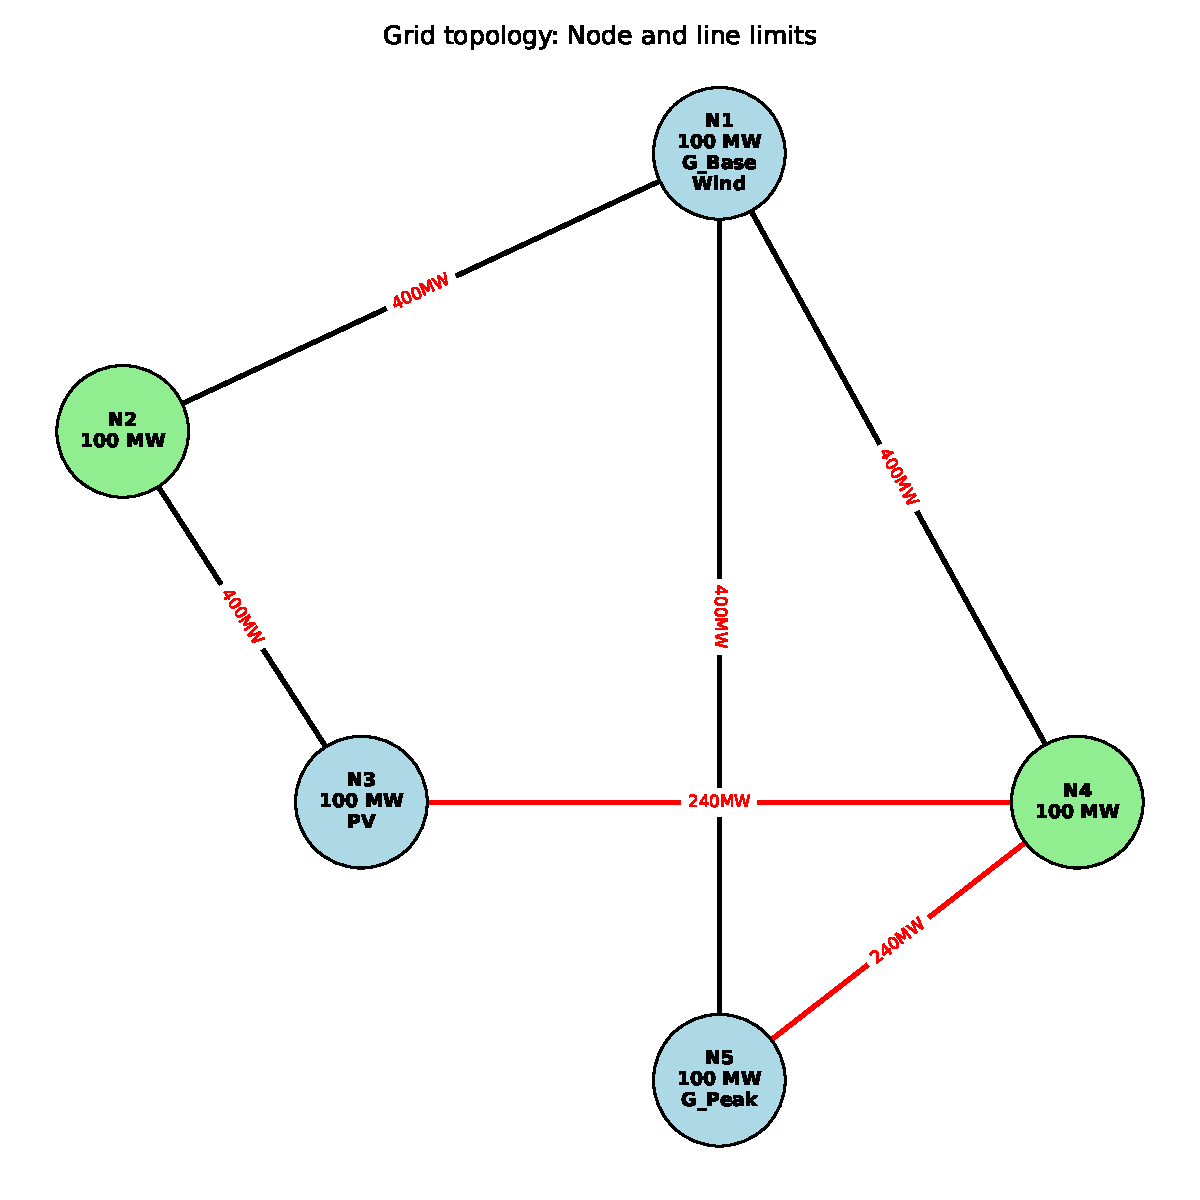
\includegraphics[width=0.75\linewidth]{figures/Figure_GridTopology.pdf}
    \caption{5-bus test system with node and line limits. G\_Base refers to the conventional generators for base load, G\_Peak refers to the conventional generators for peak load.}
    \label{fig:GridTopology}
\end{figure}

 The transmission limits of the connecting lines are strictly bounded (e.g., between 240 MW and 400 MW) to provoke network congestion, which serves as a primary driver for locational price spreads. The conventional generation fleet is divided into base-load and peak-load units, strategically placed across the nodes. To establish a distinct and realistic merit-order curve, these units are assigned specific marginal generation costs (variable costs in €/MWh). In the techno-economic parameters provided by Devine and Siddiqui \cite{devine_strategic_2023}, existing base-load units operate at approximately 48.87 €/MWh, whereas the more expensive peak-load units are assigned marginal costs of 63.38 €/MWh. For this calibrated model, the marginal generation costs are set to 40 €/MWh for base-load and 80 €/MWh for peak-load to ensure sufficient price spreads for realistic battery arbitrage.

 \subsection{Demand and Renewable Energy Profiles} \label{subsect:Profiles}
 The temporal parameters are based on real-world 24-hour profiles of the representative day 11.09.2025, extracted from Austrian TSO Austrian Power Grid (APG) data \cite{apg_generation_2025}. To observe realistic battery cycling behavior, the profiles include:
 \begin{itemize}
     \item \textbf{Load Profile}: Scaled to a system-wide peak load of 1200 MW, exhibiting a typical "duck curve" with distinct morning and evening demand peaks, as seen in Figure \ref{fig:InputLoadProfiles}. The load is spatially distributed, with 90\% concentrated in the central nodes (N2, N3, N4) and the remaining 10\% in the peripheral nodes (N1, N5).
     \item \textbf{Renewable Generation}: The model incorporates a highly volatile wind power profile with a peak capacity of 370 MW concentrated at node N1 (generating primarily at night and early morning), and a typical photovoltaic (PV) bell curve with a peak of 430 MW at node N3.
\end{itemize}

 \begin{figure}
     \centering
     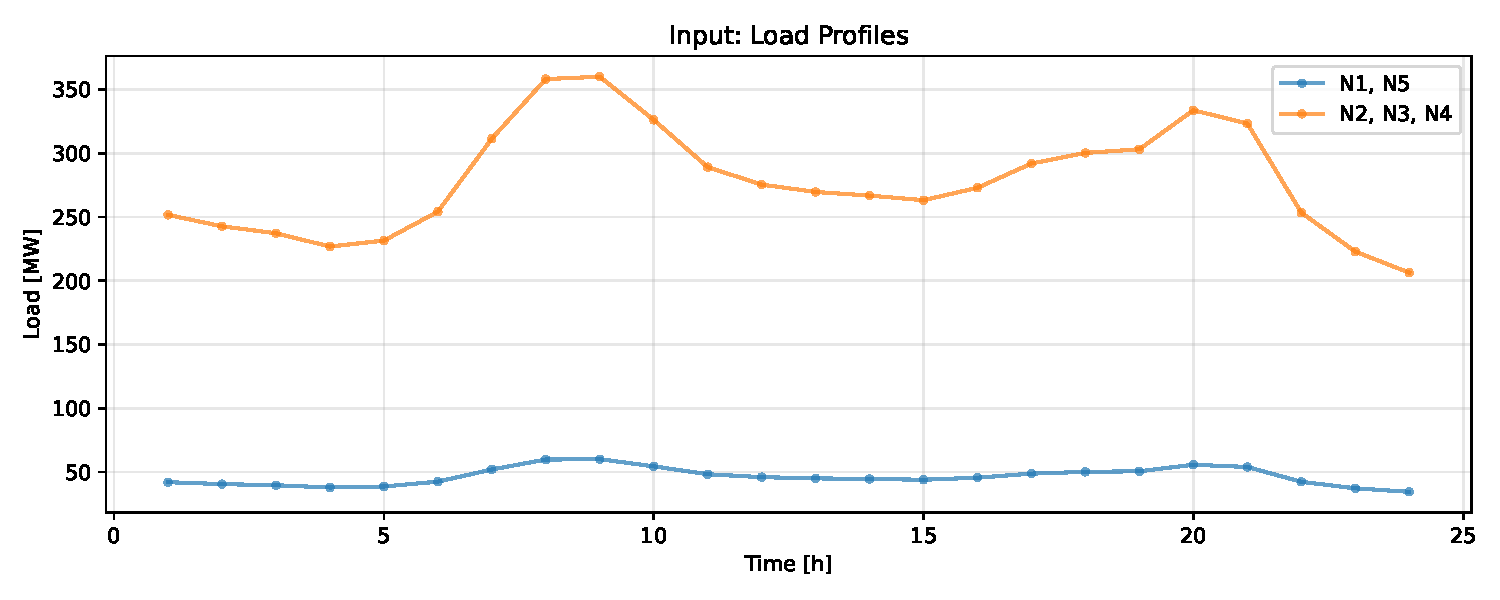
\includegraphics[width=0.75\linewidth]{figures/Figure_InputLoadProfiles.pdf}
     \caption{Load Profiles per Node.}
     \label{fig:InputLoadProfiles}
 \end{figure}
\begin{figure}
    \centering
    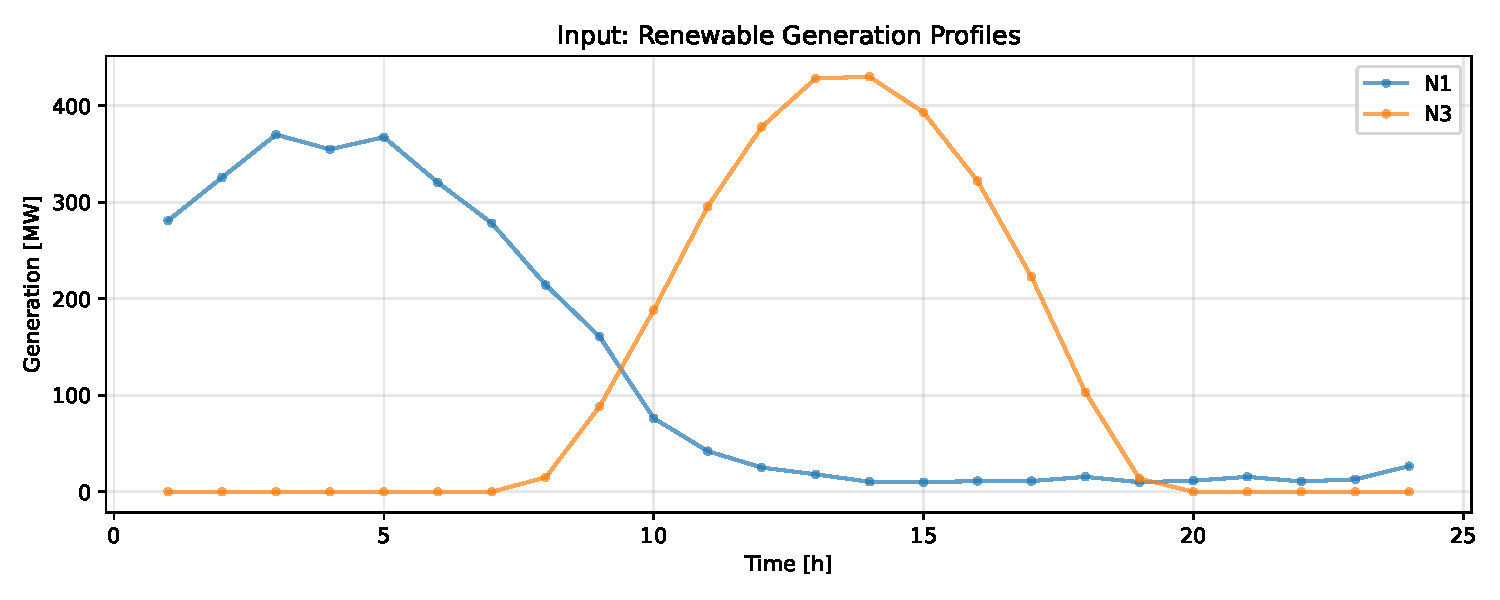
\includegraphics[width=0.75\linewidth]{figures/Figure_InputRenewableGenerationProfiles.pdf}
    \caption{Renewable Generation Profiles per Node. N1 employs Wind whereas N3 employs PV.}
    \label{fig:InputRenewableGenerationProfiles}
\end{figure}
As demonstrated by Czock et al. \cite{czock_place_2023}, the spatial discrepancy between renewable generation centers and high-demand nodes is a crucial factor for efficient storage allocation, which this empirical setup explicitly mimics.

\subsection{BESS Characteristics and Costs} \label{subsect:BESS_Characteristics}
A critical aspect of the BESS allocation problem is the correct economic assessment of the storage technology. The current literature underscores the high initial capital expenditure (CAPEX) of Lithium-Ion (Li-Ion) BESS, making accurate sizing essential for project profitability.

In this framework, the investment costs are split into power capacity costs (\(C_{power}\), representing the Power Conversion System) and energy capacity costs (\(C_{energy}\), representing the battery cells). To internalize these capital costs into the single-day optimization loop, the total CAPEX is annualized over the expected project lifetime (e.g., utilizing a 15-year horizon as common in BESS projects). Based on current techno-economic projections for utility-scale Li-Ion systems, this results in annualized daily cost parameters set at 6,600 €/MW for power and 18,800 €/MWh for energy capacity. \cite{shin_optimal_2020}.

To ensure technical feasibility and reflect realistic utility-scale storage configurations, a minimum E/P ratio constraint (\(Ratio_{min}\)) is strictly enforced at the Upper Level, as described in Equation \ref{eq:E_P_Ratio}. In this framework, the minimum E/P ratio is set to 2 hours. This establishes a balanced and widely adopted industry standard for systems performing multi-service applications \cite{das_optimal_2020, shin_optimal_2020}.

To accurately capture the physical limitations of the storage assets, several technical constants are integrated into the lower-level problem. Based on the specifications by Shin and Hur, the overall round-trip efficiency (\(\eta\)) of the BESS is modeled at 93.6\% \cite{shin_optimal_2020}.

As battery capacity degradation significantly impacts long-term profitability, the degradation penalty described in Section \ref{subsect:Battery_Degradation} is enforced. Assuming typical Li-Ion characteristics (e.g., a cycle life of 3,500 to 6,000 cycles), this is parameterized at 15 €/MWh throughput, accurately forcing the BESS to internalize its physical wear during operations.